\chapter{The geometry of legal swaps}\label{ch:swaps}

A history differs from its neighbours by exchanging adjacent independent steps. This chapter turns that observation into geometry and asks how much of the history complex can be read off the swap graph. The universal statements hold for \emph{every} set of orderings: the reconstruction of $K_A$ from the generator-coloured swap graph, and the completeness of face recognition. The statements about the \emph{uncoloured} graph hold for prefix-defined sets, and in a verified range of $k$.

\section{Squares, hexagons and generator colours}
The permutohedron graph is the Cayley graph of $S_k$ for $s_1,\dots,s_{k-1}$, where $x\mapsto xs_i$ exchanges the entries in positions $i,i{+}1$; the edge $\{x,xs_i\}$ has \emph{colour} $i$. The Coxeter relations $s_i^2=e$, $(s_is_j)^2=e$ for $|i-j|\ge2$ (a commuting pair) and $(s_is_{i+1})^3=e$ (a braid relation) give the two kinds of $2$-faces: a \emph{square} $x\langle s_i,s_j\rangle$ ($|i-j|\ge2$, four vertices) and a \emph{hexagon} $x\langle s_i,s_{i+1}\rangle$ (six vertices). For $J\subseteq\{1,\dots,k-1\}$ let $W_J=\langle s_j:j\in J\rangle$, a product of symmetric groups on the maximal runs of consecutive positions.

@@lem:parabolic@@

\begin{figure}[ht]\centering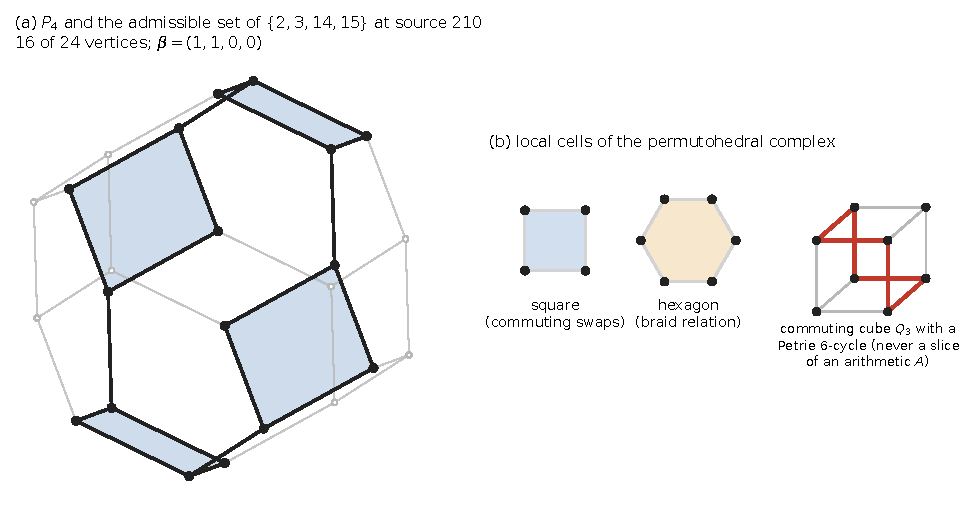
\includegraphics[width=\textwidth]{figures/fig_swap_geometry.pdf}
\caption{Legal-swap geometry. (a) The permutohedron $P_4$ (a truncated octahedron, orthographic projection of the exact vertex coordinates): the sixteen admissible histories of content $\{2,3,14,15\}$ at source $210$, their twenty legal swaps and the four square faces of $K_A$. The loop through the hexagonal region is not filled, so $\beta=(1,1,0,0)$. (b) The two kinds of $2$-cells, and a commuting cube with a Petrie $6$-cycle (red), which cannot be the trace of a prefix-defined set (\cref{cor:CP}).}\label{fig:swaps}
\end{figure}

\section{Reconstruction from the coloured swap graph}
@@thm:swap-reconstruction@@
@@prop:iso-profiles@@

\section{What the uncoloured graph determines}\label{sec:graph-only}
Without colours, additional structure is needed. For every $k$ the squares are visible:
@@lem:four-cycles@@
Six-cycles require a classification that is available for a finite range.
@@lem:six-cycles+computer-assisted@@
The adjacency claim for braid hexagons holds for all $k$:
@@lem:braid-isolated@@
@@thm:skeleton+computer-assisted for $k\le8$@@
@@prop:petrie@@
\Cref{cor:CP} shows that no prefix-defined set has a Petrie cycle as the trace of a cube without its antipodes, which is exactly why graph-only recovery works for arithmetic systems.

\section{Recognising higher cells}
Beyond dimension two, cells are recognised by convexity.
@@thm:face-recognition@@
@@thm:third-boundary@@
Whether graph-isomorphic realizable pairs with different homology exist at all reduces to part (d) of \cref{thm:face-recognition}; none was found in the verified domains.
